\documentclass{article}

\usepackage{graphicx}
\usepackage{amsmath}
\usepackage[a4paper,total={7in, 10in}]{geometry}
\setlength{\parindent}{0pt}

\title{Anita's document extra help}
\author{Roberto Alvarado}
\begin{document}
\maketitle
The first image in the notebook is just a candle bar with the information of the
local highs and the local lows in order to get the channels of the stock
\begin{figure}[h]
  \caption{First image}
  \begin{center}
    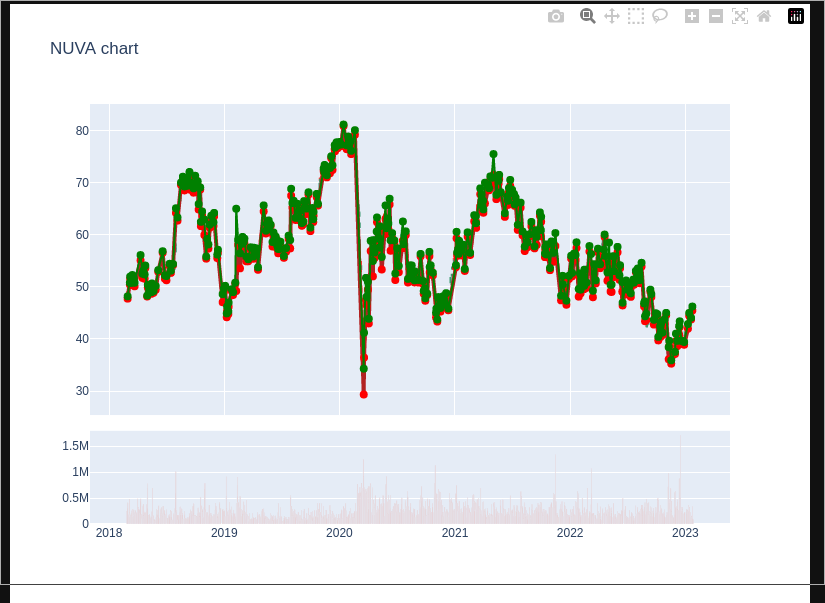
\includegraphics[width=0.5\textwidth]{figures/2.png}
  \end{center}
\end{figure}
In this image, each point represent the relation of the price of the stock and
how many days it took to reach again that point again. You can see that there
are many higher priced moments that took a lot of time to reach again, that
could be consider as local highs!, they reach that point and the went down bad 
\begin{figure}[h]
  \caption{Relation between price and time to recover}
  \begin{center}
    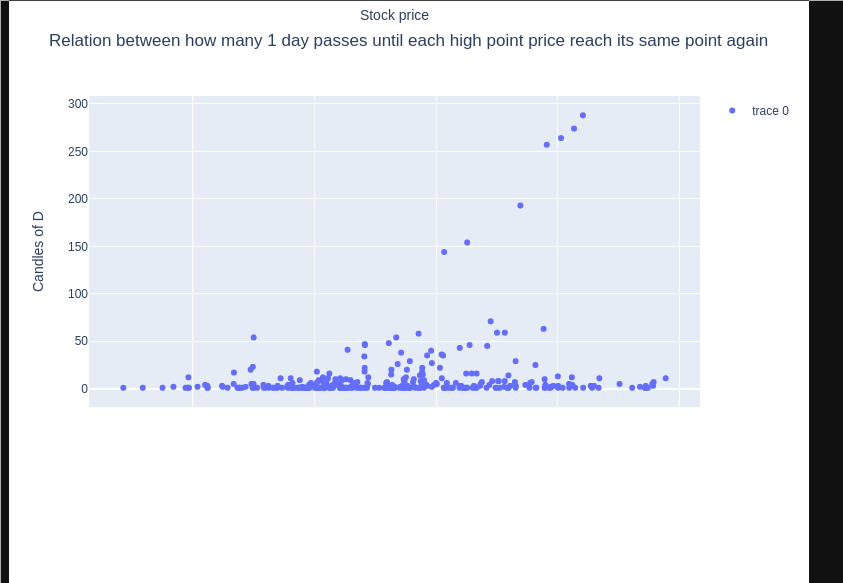
\includegraphics[width=0.5\textwidth]{figures/1.png}
  \end{center}
\end{figure}
\newpage
In the next group of figures we see the relation between many parameters and the
number of channels.

First in this figure we see the relation of the quantity channels and the
volume that is traded, in this case we see clearly that there are a lot more
channels that transaction in with little volumes, but are many that push the
average forward
\begin{figure}[h]
  \caption{Relation between volume and number of channels}
  \begin{center}
    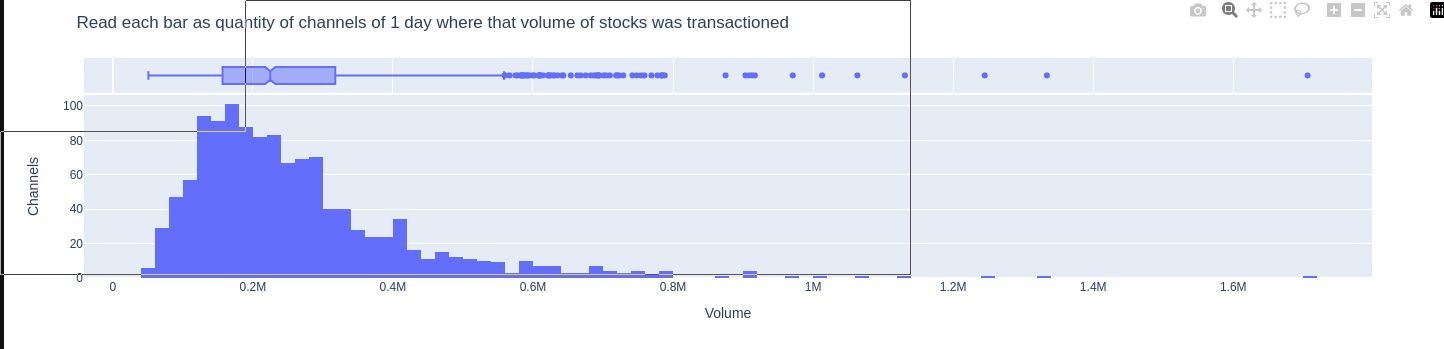
\includegraphics[width=0.8\textwidth]{figures/2023-05-25-142825_1444x349_scrot.png}
  \end{center}
\end{figure}

In this graph we see  how many channels have in relation of the slope change of
highs and lows. The next graph is the same but for highs. For example, in the
lows graphs, we can see there is a normal distribution with a negative bias,
meaning that it is bigger on the right! Meaning there are more channels that
have a positive change on their lows, but the average as it is expected is 0.
\begin{figure}[h]
  \caption{Highs \% change}
  \begin{center}
    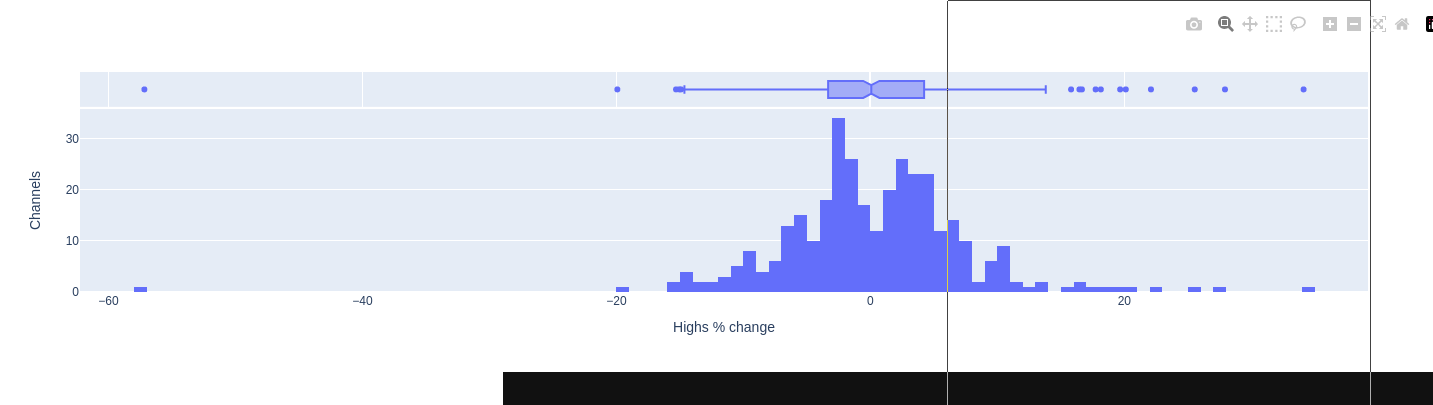
\includegraphics[width=0.8\textwidth]{figures/5.png}
  \end{center}
\end{figure}
\begin{figure}[h]
  \caption{Lows \% change}
  \begin{center}
    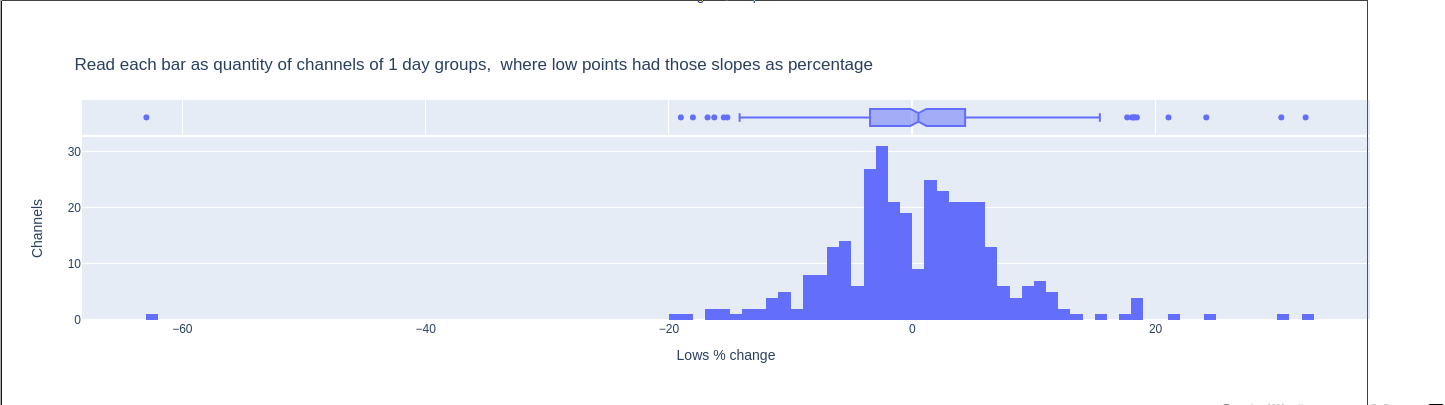
\includegraphics[width=0.8\textwidth]{figures/4.png}
  \end{center}
\end{figure}
\newpage
In this new set of figures start a stronger analysis of the slopes of the
channels, first we can see all data grouped
\begin{figure}[h]
  \caption{Complete analysis}
  \begin{center}
    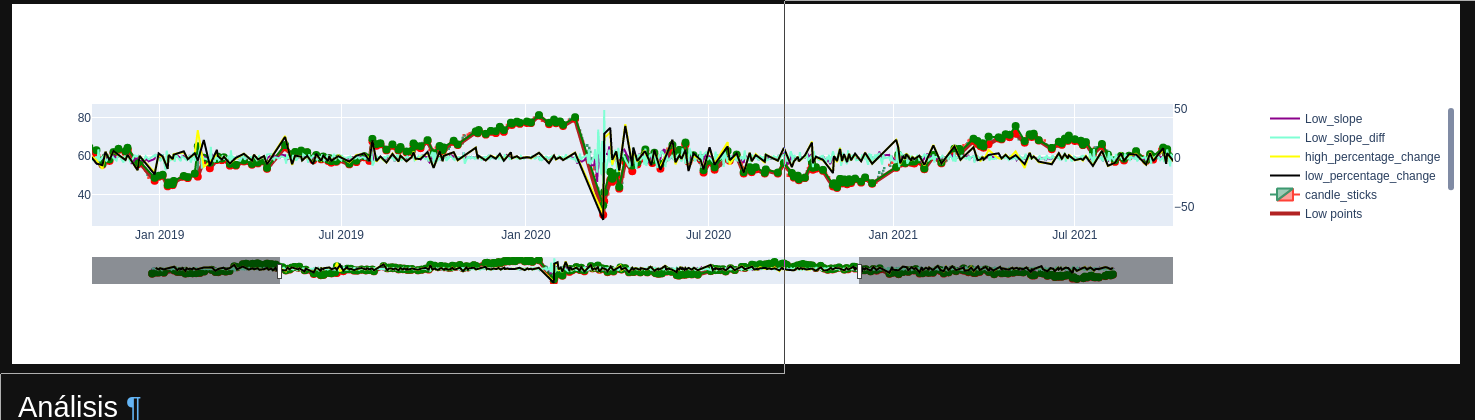
\includegraphics[width=1\textwidth]{figures/2023-05-25-143714_1475x420_scrot.png}
  \end{center}
\end{figure}
For Figure 6, first is important to explain each of the parts of the graph, the
green and red lines are as in Figure 1, so is not that important, we see the
black lines that represent the change beetween the lows at the start and the end
of each of the channels, a positive slope of this means that there is an
increment in price at the end of the channel. Same idea for the yellow line but
for the highs.
\begin{figure}[h]
  \caption{Complete analysis}
  \begin{center}
    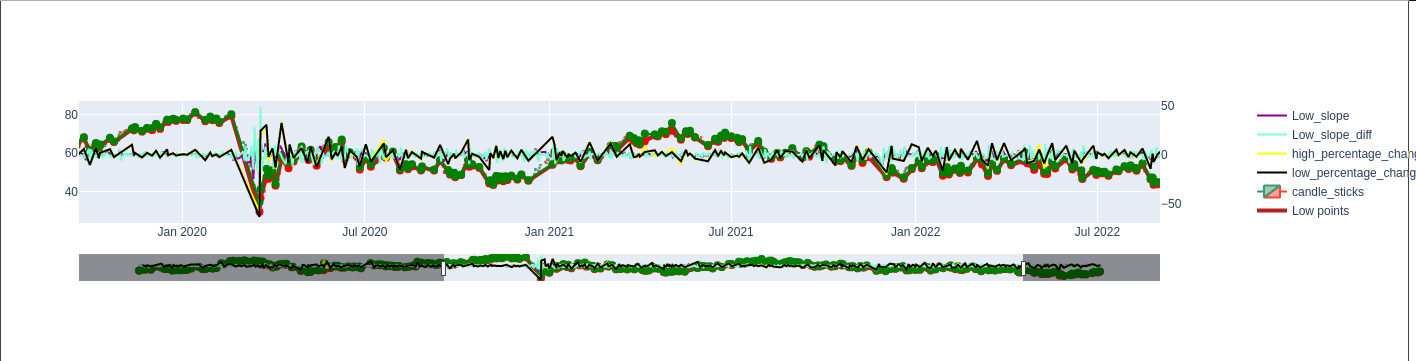
\includegraphics[width=1\textwidth]{figures/2023-05-25-143658_1416x361_scrot.png}
  \end{center}
\end{figure}

With this clarification we can start making some analysis, for example, in the
next paragraph can be a result based on this graph.

\textit{Example of Possible  Analysis}

There is an instance that can demonstrate how a positive drop in the low is reflected (JAN-2020 and JUL-2020). There is a positive slope again, almost like a regulator where it returns to a similar price.
It seems to regulate itself in a certain way with these extreme drops. When it grows too much, it will try to fall. However, with the drop, this changes. If the price starts to decrease, there is an almost one-year period where it returns to an average value (just an idea of an average value). So it is easy for it to fall to the bottom, but difficult for it to rise when it falls.

\begin{figure}[h]
  \caption{Section for analysis}
  \begin{center}
    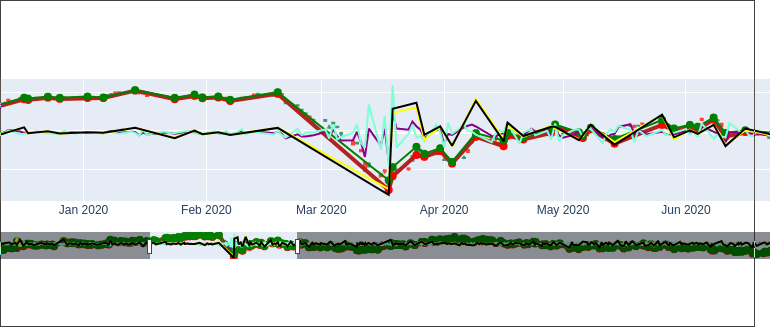
\includegraphics[width=0.5\textwidth]{figures/2023-05-25-144607_770x329_scrot.png}
  \end{center}
\end{figure}
\newpage
In this case we are going to focus on channel size, as this image see the
relation between the low's change and channel size. We could make a statement as  there seems to be no linear relationship between the size of the channels and the percentage drops in the low. There is a case where it can be observed that there is a very large channel, specifically with 20 tickers, and here the change in the low is substantial. However, further analysis would be needed to consider it an outlier. An important insight is that after the channel has been active for 5 days, the change becomes much more prominent, whether it is an upward or downward movement. The key point is to note that there is more variation.
\begin{figure}[h]
  \caption{Relation between size channel and low change}
  \begin{center}
    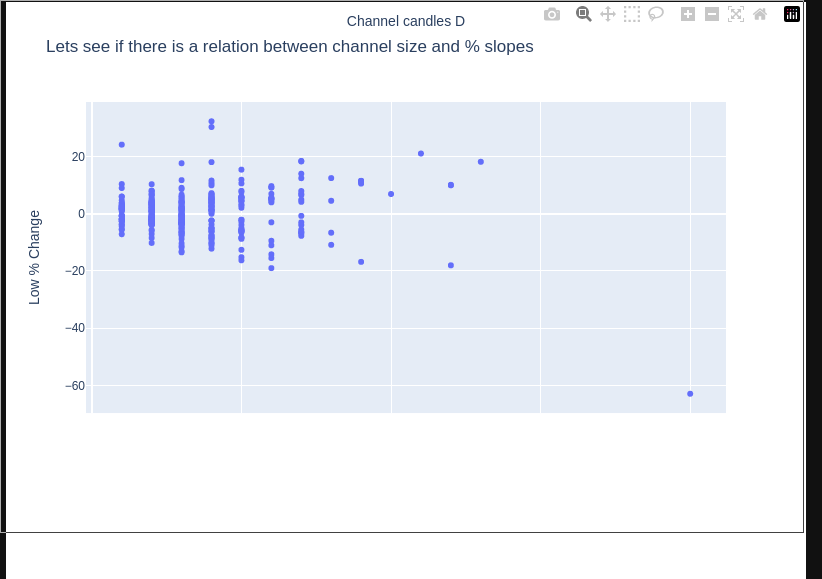
\includegraphics[width=0.5\textwidth]{figures/10.png}
  \end{center}
\end{figure}
In Figure 10, we make a graph to show the relationship between the size of
channels and the size of previous and next channel.In this case, the same pattern can be observed as in other interpretations. If you notice, there isn't a noticeable relationship among the cases. However, it can be seen that compared to the current channels, the previous channels exhibit much more variation. We can once again observe the outlier in our sample.
\begin{figure}[h]
  \caption{Past and previous channel change}
  \begin{center}
    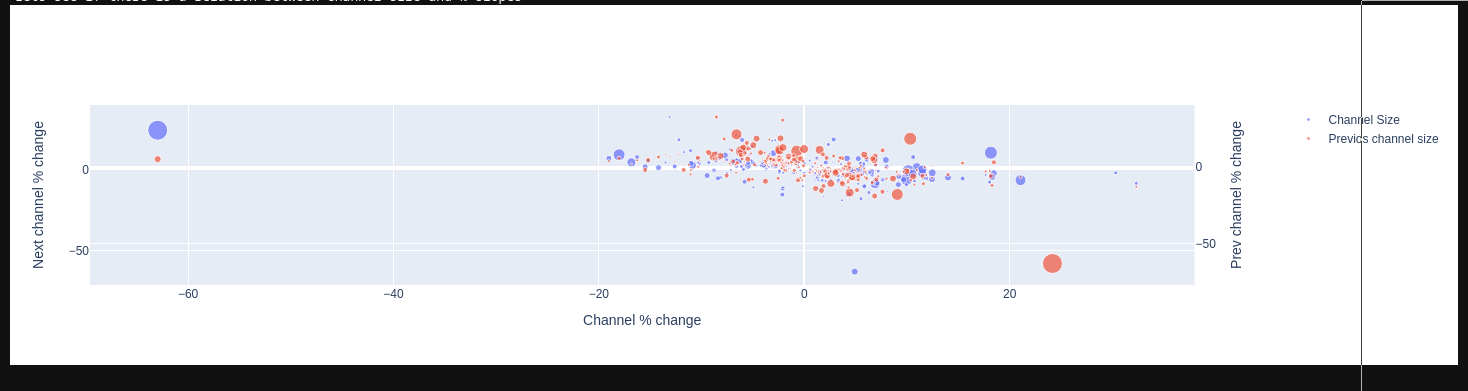
\includegraphics[width=0.8\textwidth]{figures/11.png}
  \end{center}
\end{figure}
\newpage
In this case we can see the relation between the size of the previous channel
size and the current change of the price of the channel, we could make an
assumption based on the data, as it was noticed by ANITA. If the previous channel had a duration equal to or greater than ten business days, it is likely that the current channel will exhibit positive variation, regardless of the direction of the previous channel.
\begin{figure}[h]
  \caption{Past and channel size change}
  \begin{center}
    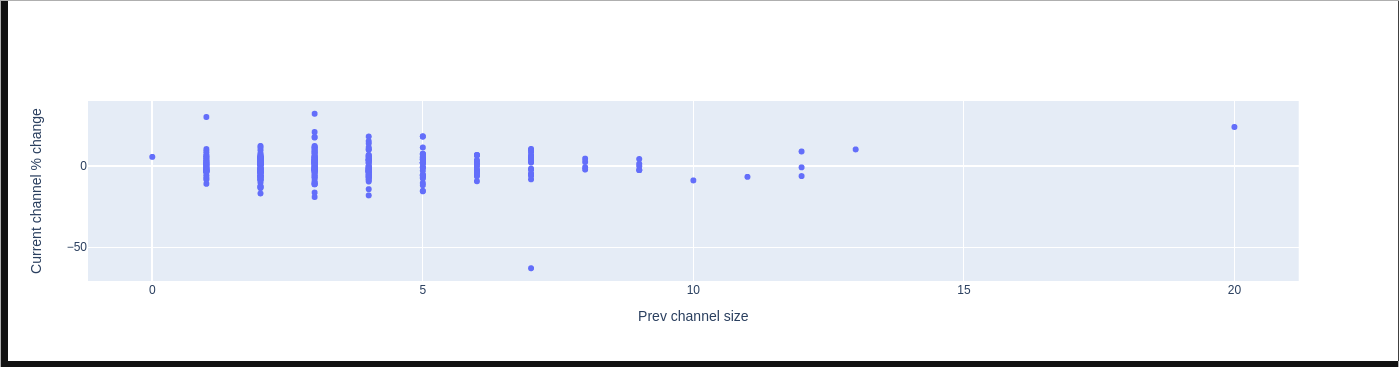
\includegraphics[width=0.9\textwidth]{figures/12.png}
  \end{center}
\end{figure}

Now we enter the analysis of consolidation points. We want to focus on the next
question.

Definition of consolidation: percentage change of the channel close to zero. When the slopes are within these ranges, what is the common variation of the subsequent and previous channels?
\begin{figure}[h]
  \caption{Relation between next channel and number of consolidated channels}
  \begin{center}
    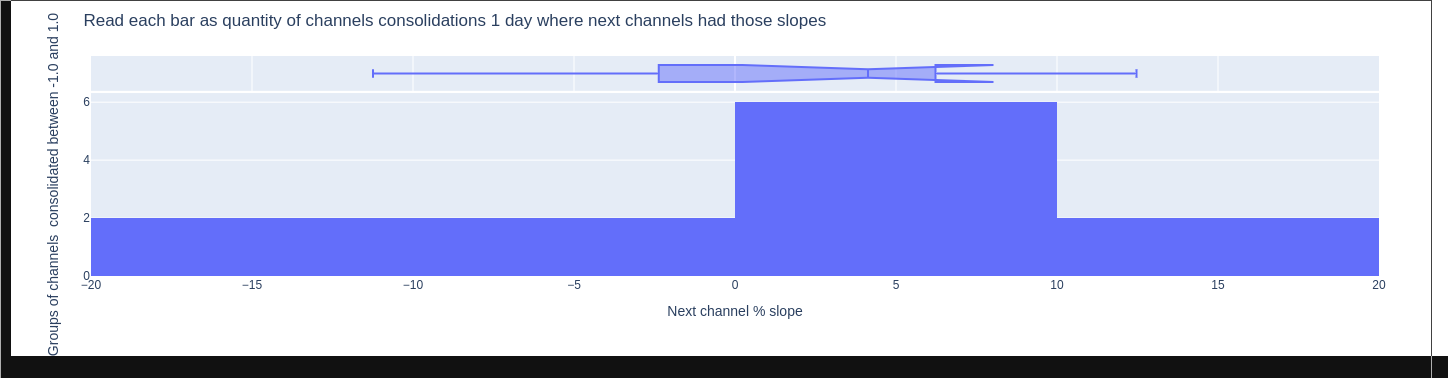
\includegraphics[width=0.8\textwidth]{figures/13.png}
  \end{center}
\end{figure}

In Figure 12, we see the relationship of the slope or change of the next channel
and how many of the channels consolidated between 1\% to +1\%. In it can be
observed that there are more channels where the channel 
had a growth. This means that if a channel consolidation occurs within the range
of -1\% to +1\%, it is feasible to expect that its low will experience growth.

In Figure 13, is the same properties but for the previous channel, a little
insight could be that 
In this case, the opposite happens compared to the subsequent days. Here, there
is a tendency that if the channel consolidates within the range of -1\% to +1\%, then the channel tends to fall with a negative slope.
\begin{figure}[h]
  \caption{Relation between previous channel and number of consolidated channels}
  \begin{center}
    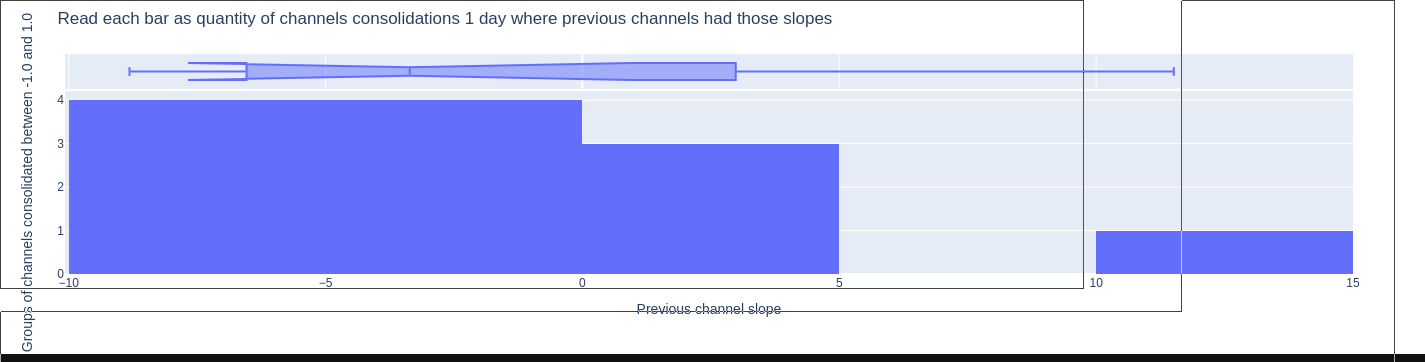
\includegraphics[width=0.8\textwidth]{figures/14.png}
  \end{center}
\end{figure}
\newpage
In this next figure we could see where the consolidation points appear. We could
see a little insight of this graph. As there is a clear trend throughout the
channels to return to stabilization around the value of 60, as every time there
is a channel with a significant growth, it starts to decline rapidly. As we can
see from the beginning of 2021, this growth stabilized, and now it is at a
historical low (excluding 2020, which could be considered a reflection of the
pandemic). The consolidation points are a good way to understand it. The first
consolidation point in 2022 is higher than the subsequent ones, but the sampling
shows that there could be an increase in the coming months.
\begin{figure}[h]
  \caption{Conciliation points}
  \begin{center}
    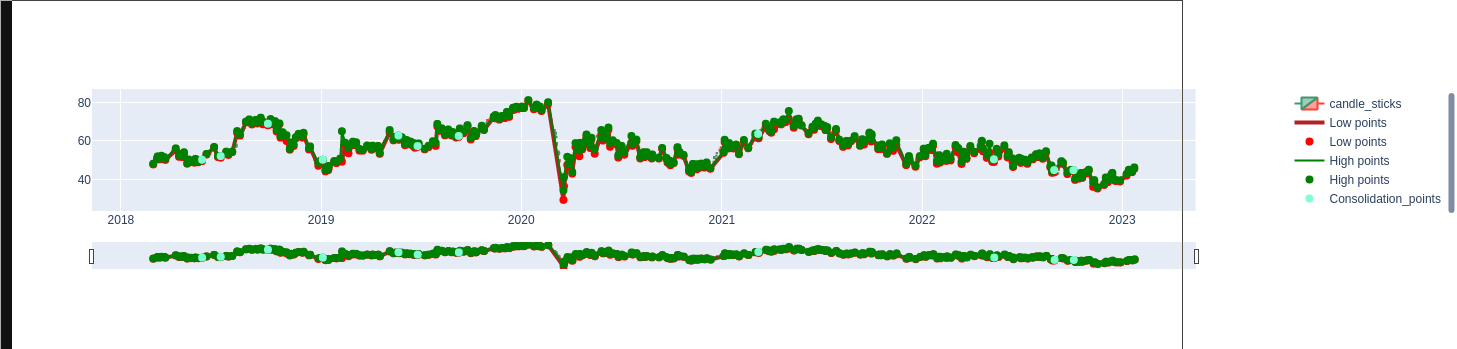
\includegraphics[width=0.9\textwidth]{figures/15.png}
  \end{center}
\end{figure}

Now from this point forward we are going to analyse the following theory

Loopa Technologies theory: Whenever there is a high positive change between the slopes of the channels, it is a good entry point.

For the first Figure (15) we are going to see the relation between how many
candles are and the change of the slope of the lows between them.
The normal curve obtained is simply a reflection of a normal distribution, which can be expected from a process that doesn't have any manageable trend but only a normal relationship between changes in slopes and their magnitudes. However, there is a negative bias, indicating a slight tendency towards tickers with positive changes.
\begin{figure}[h]
  \caption{Section for analysis}
  \begin{center}
    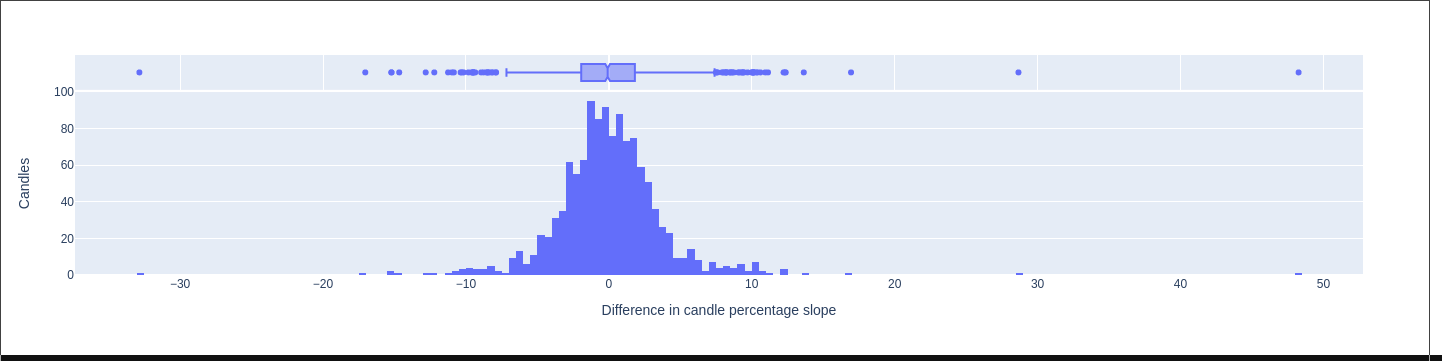
\includegraphics[width=0.9\textwidth]{figures/16.png}
  \end{center}
\end{figure}
\newpage
First explaining the graph, purple dots are the slope variations between
channels, yellow define the channel size variation between channels. The other
parts are simply from past graphs. We could make an analysis.

The yellow dots represent the percentage variation of the channels, which can be seen as a good growth indicator, as mentioned by Anita. However, the slope changes, represented by the purple dots, as expected, have a higher correlation with price. For example, if there is a case where there are three slope variations following the order: the first one lower than the second, and the second one higher than the third, it seems that there is a decline in the stock. A more comprehensive analysis should be conducted to determine if this can be considered a viable strategy.
\begin{figure}[h]
  \caption{Section for analysis}
  \begin{center}
    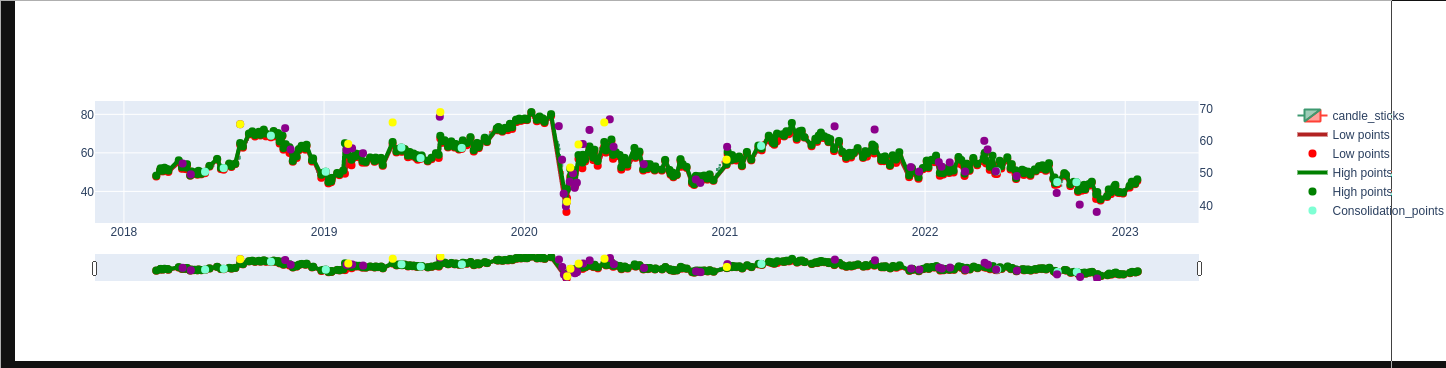
\includegraphics[width=0.9\textwidth]{figures/17.png}
  \end{center}
\end{figure}

In this final figure we could see how many candles are for the difference
between the highs and lows of the candle. In this case,
a normal distribution with a positive skew is evident. It is clear that there is a mean around 0, but there is a greater tendency for the differences to be negative.
\begin{figure}[h]
  \caption{Section for analysis}
  \begin{center}
    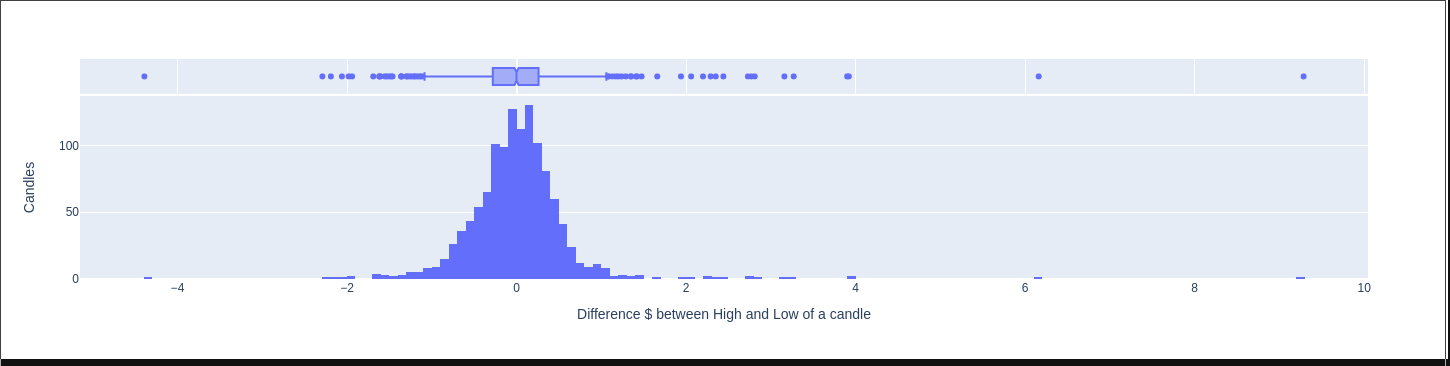
\includegraphics[width=0.9\textwidth]{figures/18.png}
  \end{center}
\end{figure}
\end{document}
